\subsection{Completed experiments and performance}

All ten outer partitions completed: 500 candidate fits, 50 selected model fits, and ten constant-reference evaluations. The exported metrics contain 60 evaluated model/protocol/seed combinations. Automated checks recompute metrics from predictions, verify labels against source records, and verify partition integrity. No convergence warnings were observed in the completed-run logs. Table~\ref{tab:performance} and Fig.~\ref{fig:comparison} summarize the main results. Values are preliminary benchmark findings, not clinical validation.

\begin{table}[t]\caption{Test performance, mean $\pm$ sample SD across five seeds. Constant AP equals each test set\textquotesingle s positive fraction.}\label{tab:performance}\centering\footnotesize\begin{tabular}{llcc}\toprule Model & Split & AP & ROC-AUC\\\midrule

L2 logistic & Patient & 0.216 $\pm$ 0.006 & 0.663 $\pm$ 0.003 \\

L2 logistic & Encounter & 0.221 $\pm$ 0.002 & 0.669 $\pm$ 0.005 \\

L1 logistic & Patient & 0.215 $\pm$ 0.006 & 0.665 $\pm$ 0.003 \\

L1 logistic & Encounter & 0.222 $\pm$ 0.002 & 0.671 $\pm$ 0.004 \\

Random forest & Patient & 0.208 $\pm$ 0.002 & 0.665 $\pm$ 0.005 \\

Random forest & Encounter & 0.221 $\pm$ 0.002 & 0.673 $\pm$ 0.004 \\

LightGBM & Patient & 0.228 $\pm$ 0.006 & 0.673 $\pm$ 0.002 \\

LightGBM & Encounter & 0.238 $\pm$ 0.004 & 0.679 $\pm$ 0.003 \\

L2 unweighted & Patient & 0.216 $\pm$ 0.006 & 0.662 $\pm$ 0.003 \\

L2 unweighted & Encounter & 0.221 $\pm$ 0.002 & 0.668 $\pm$ 0.005 \\

Constant & Patient & 0.112 $\pm$ 0.002 & 0.500 $\pm$ 0.000 \\

Constant & Encounter & 0.114 $\pm$ 0.000 & 0.500 $\pm$ 0.000 \\

\bottomrule\end{tabular}\end{table}

\begin{figure}[t]\centering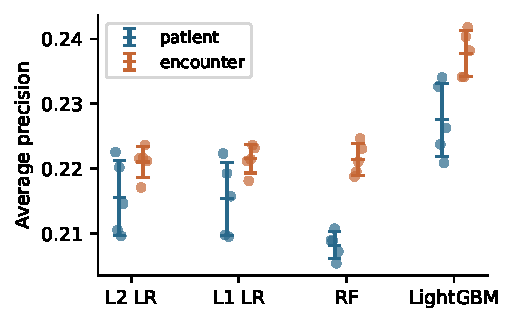
\includegraphics[width=\columnwidth]{comparison.pdf}\caption{AP across five seeds. Points are individual runs; marks and error bars show means and sample standard deviations.}\label{fig:comparison}\end{figure}

LightGBM has the highest mean patient-level AP (0.228), compared with 0.216 for weighted L2 and 0.112 for the constant reference. The encounter-minus-patient differences in mean AP are +0.0055 (L2 logistic), +0.0062 (L1 logistic), +0.0132 (Random forest), +0.0102 (LightGBM). These are descriptive differences across separately constructed test sets. They are not paired causal effects of overlap.

\subsection{Overlap and conditional uncertainty}

Patient-level holdouts have zero patient overlap by assertion. Encounter-level overlap ranges from 41.34\% to 42.10\% of test encounters (mean 41.70\%). Patient-arm test prevalence ranges from 10.99\% to 11.41\%; the corresponding test sizes range from 19,717 to 19,991. The constant-reference results make this variation explicit.

For LightGBM within encounter-level holdouts, mean AP is 0.279 for seen patients and 0.157 for unseen patients. Their mean positive fractions are 20.10\% and 5.16\%, respectively. The case-mix and prevalence difference prevents interpreting this subset contrast as an isolated overlap effect.

For the prespecified patient holdout at seed 42, paired AP differences relative to weighted L2 and their 95\% patient-bootstrap intervals are L1 logistic: -0.0010 [-0.0026, +0.0006]; Random forest: -0.0095 [-0.0169, -0.0021]; LightGBM: +0.0138 [+0.0073, +0.0214]. These conditional, unadjusted intervals complement rather than replace the repeated-seed summaries.

\subsection{Thresholds and probability quality}

\begin{table}[t]\caption{Patient-level threshold and probability diagnostics: means across five runs. Thresholds maximize development out-of-fold F1.}\label{tab:diagnostics}\centering\footnotesize\begin{tabular}{lrrrr}\toprule Model & Precision & Recall & F1 & Brier\\\midrule

L2 logistic & 0.193 & 0.475 & 0.274 & 0.225\\

L1 logistic & 0.193 & 0.476 & 0.275 & 0.225\\

Random forest & 0.189 & 0.500 & 0.274 & 0.219\\

LightGBM & 0.211 & 0.435 & 0.284 & 0.215\\

L2 unweighted & 0.197 & 0.447 & 0.272 & 0.095\\

Constant & 0.000 & 0.000 & 0.000 & 0.099\\

\bottomrule\end{tabular}\end{table}

Table~\ref{tab:diagnostics} reports the precision--recall trade-off after development-only threshold selection. Unweighted L2 has mean Brier score 0.095, compared with 0.225 for weighted L2. The calibration diagnostic (Fig.~\ref{fig:calibration}) illustrates why class-weighted scores should not automatically be interpreted as calibrated risks. Brier score combines discrimination and calibration; a lower value alone does not establish perfect calibration. No probability correction has yet been fitted.

\begin{figure}[t]\centering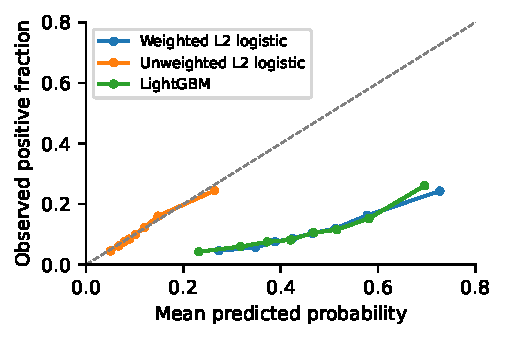
\includegraphics[width=\columnwidth]{calibration.pdf}\caption{Calibration diagnostic for the prespecified patient holdout, seed 42. Eight quantile bins; dashed line indicates ideal calibration. This is a diagnostic, not a fitted correction.}\label{fig:calibration}\end{figure}
